\thispagestyle{empty}\SourceLeaf{002}
\vspace*{1in}
\begin{center}
{\Large\bfseries CARL FRIEDRICH GAUSS WORKS\par}
\vspace{.45in}
{\large\bfseries VOLUME IV.\par}
\end{center}
\clearpage
\thispagestyle{empty}\SourceLeaf{004}
\begin{center}
{\Large\bfseries CARL FRIEDRICH GAUSS\par}
\vspace{.25in}
{\Huge\bfseries WORKS\par}
\vspace{.3in}
{\large\bfseries FOURTH VOLUME.\par}
\vspace{.4in}
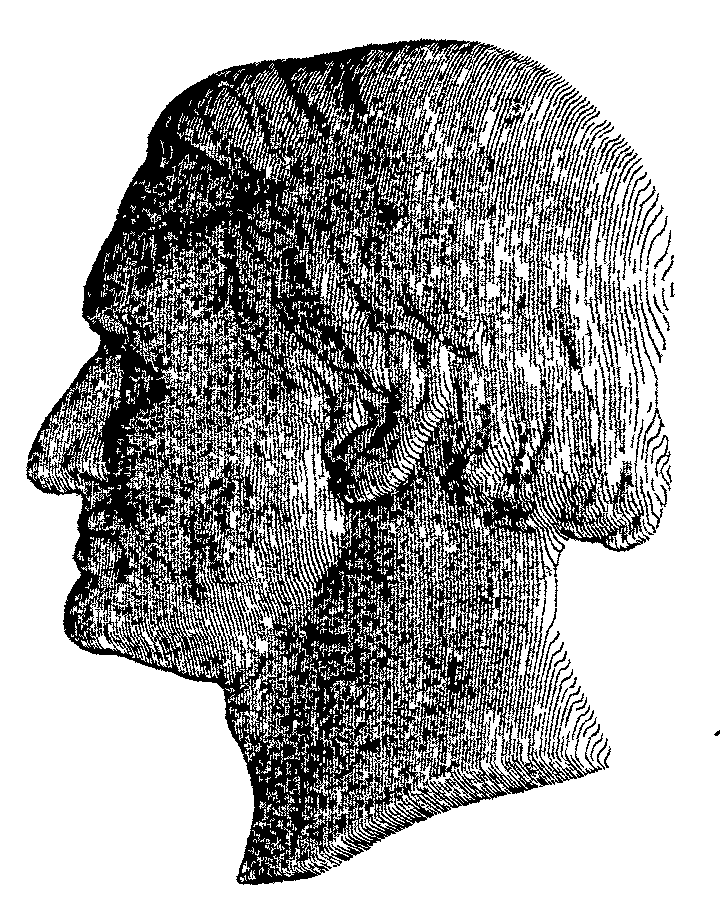
\includegraphics[height=2.45in]{assets/native004_original_portrait.png}
\vspace{.4in}

{\small EDITED\par}
\medskip
{\small BY THE\par}
\medskip
{\normalsize ROYAL SOCIETY OF SCIENCES\par}
\smallskip
{\small AT\par}
\medskip
{\large GÖTTINGEN\par}
\smallskip
1873.
\end{center}
\clearpage
\thispagestyle{empty}\SourceLeaf{006}
\begin{center}
\vspace*{.25in}
{\Large THEORY\par}
\vspace{.3in}
{\Large\bfseries OF THE COMBINATION OF OBSERVATIONS\par}
\vspace{.2in}
{\large SUBJECT TO THE SMALLEST ERRORS\par}
\vspace{.4in}
{\large FIRST PART\par}
\vspace{.45in}
{\small BY\par}
\vspace{.3in}
{\large CARL FRIEDRICH GAUSS\par}
\vspace{.45in}
{\small PRESENTED TO THE ROYAL SOCIETY OF SCIENCES 1821. FEBR. 15.\par}
\vspace{.4in}
\rule{.9\linewidth}{.3pt}\par
\smallskip
{\small Commentationes societatis regiae scientiarum Gottingensis recentiores. Vol.\,v.\par}
\smallskip
{\small Göttingen \textsc{mdcccxxiii}.\par}
\smallskip
\rule{.9\linewidth}{.3pt}
\end{center}
\clearpage
\SourceLeaf{008}
\begin{center}
{\large THEORY\par}
\medskip
{\Large\bfseries OF THE COMBINATION OF OBSERVATIONS\par}
\medskip
{\large SUBJECT TO THE SMALLEST ERRORS.\par}
\medskip
{\large\textsc{First Part.}\par}
\medskip
\rule{.22\linewidth}{.3pt}
\end{center}
\Article{1}
However much care is taken in making observations concerned with the magnitudes of natural things, they nevertheless always remain subject to larger or smaller errors. Errors of observation are usually not simple, but arise from several sources at once: two kinds of these sources must be carefully distinguished. Some causes of error are such that their effect in any observation depends on variable circumstances between which and the observation itself no essential connection is understood: the errors arising from these causes are called irregular or random, and insofar as those circumstances cannot be subjected to calculation, the same holds for the errors themselves. Such are the errors arising from the imperfection of the senses, and also from irregular external causes, e.g. the quivering motion of the air, which slightly disturbs vision: several defects of even the best instruments must also be included here, e.g. roughness of the inside of spirit levels, lack of absolute stability, etc. Other causes of error, by contrast, by their nature produce in all observations of the same kind an effect that is either absolutely constant, or at least one whose magnitude depends, according to a definite law, solely on circumstances regarded as essentially connected with the observation. Errors of this kind are called constant or regular.

It is evident, moreover, that this distinction is relative to some extent, and depends on the wider or narrower sense in which the notion of observations belonging to the same kind is taken. For example, irregular defects in the graduation of instruments for measuring \SourceLeaf{009}angles produce a constant error whenever the question is merely one of repeating the observation of a particular angle indefinitely, since the same faulty divisions are always used in this case: on the other hand, the error arising from this source can be regarded as random whenever the question is indefinitely one of measuring angles of any magnitude, provided there is no table showing the amount of error in the individual divisions.

\Article{2}
Strictly speaking, the consideration of regular errors is excluded from our purpose. It is the observer's task to investigate diligently all causes capable of producing constant errors, and either to remove them, or at least to examine their nature and magnitude with the utmost care, so that their effect can be determined in any particular observation. The observation can thus be freed from that effect, which amounts to the same thing as if the error had not been present at all. The situation is very different, however, with irregular errors, which by their nature cannot be subjected to calculation. These must therefore be tolerated in the observations, but their effect on the quantities to be derived from the observations must be reduced as much as possible by a skilful combination of the latter. The following investigations are devoted to this most important subject.

\Article{3}
Errors in observations belonging to the same kind that arise from a particular simple cause are, by the nature of the matter, confined within certain \textit{limits}, which could undoubtedly be assigned exactly if the nature of the cause itself were \textit{fully} understood. Most causes of random errors are such that, according to the law of continuity, all errors contained within those limits must be regarded as possible, and perfect knowledge of the cause would also teach us whether all these errors are equally likely or not equally likely. In the latter case it would also teach us what relative probability is to be assigned to each error. The same will hold for the total error, compounded from several simple errors: namely, it will be enclosed within certain limits, (one of which will be equal to the sum of all the partial upper limits, the other to the sum of all the lower limits); all errors within these limits will indeed be possible, but since each can be composed in infinitely many different ways from partial errors that are themselves more or less probable, we shall have to assign a greater chance to one and a smaller chance to another, and the law of rela\SourceLeaf{010}%
tive probability can be found if the laws of the simple errors are assumed known, subject to the analytical difficulties of collecting all the combinations.

There are, indeed, some causes of error that can produce only discrete errors, rather than errors proceeding according to the law of continuity, such as errors in the graduation of instruments, (if one chooses to count these among random errors): for the number of divisions in any particular instrument is finite. It is evident, however, that notwithstanding this, provided that not all the causes of error produce discrete errors, the collection of all possible total errors will constitute a series proceeding according to the law of continuity, or several such interrupted series if, when all possible discrete errors are arranged in order of magnitude, one or another difference between two adjacent terms happens to be greater than the difference between the limits of the total errors insofar as they arise from continuous errors alone. But in practice the latter case will hardly ever occur, unless the graduation suffers from rather gross defects.

\clearpage
